\subsection{Prototypes}
To come to a common vision about the layout and functionality of the system, a series of prototypes were created.
The primary focus of these prototypes is not to be used for implementation, but rather for comparing opinions about how the flow in the system should be created.

Since the user interface is mostly focused on the mobile devices that the players will be wearing, it was decided that the host computer should simply be provided by a text-based interface, as seen on \autoref{fig:prototype:hostlobby}.

\begin{figure}[H]
    \centering
    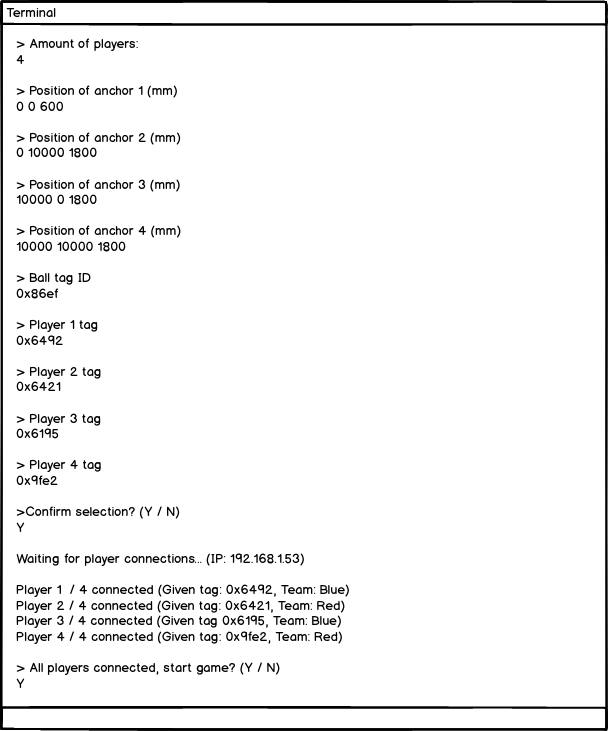
\includegraphics[width=0.6\linewidth]{prototypes/hostlobby.png}
    \caption{Prototype of hosting interface}
    \label{fig:prototype:hostlobby}
\end{figure}

When a user starts the application, they will be greeted with an input field, where they will specify the IP address of the host machine, as seen on \autoref{fig:prototype:menu}. 

\begin{figure}[H]
    \centering
    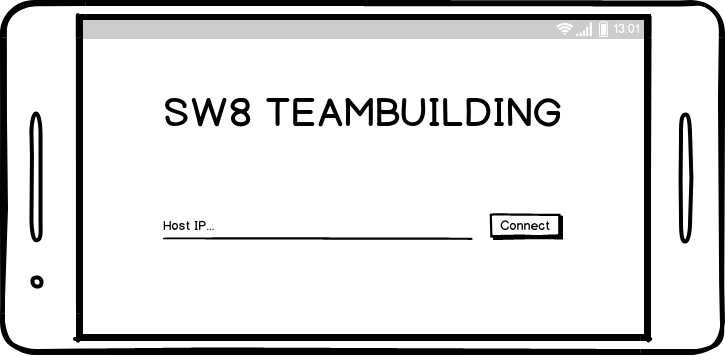
\includegraphics[width=0.6\linewidth]{prototypes/menu.png}
    \caption{Prototype of game menu}
    \label{fig:prototype:menu}
\end{figure}

After inputting an IP and confirming, they will be redirected to a page where they can see how many users have connected to the host, as seen on \autoref{fig:prototype:menuconnected}. 

\begin{figure}[H]
    \centering
    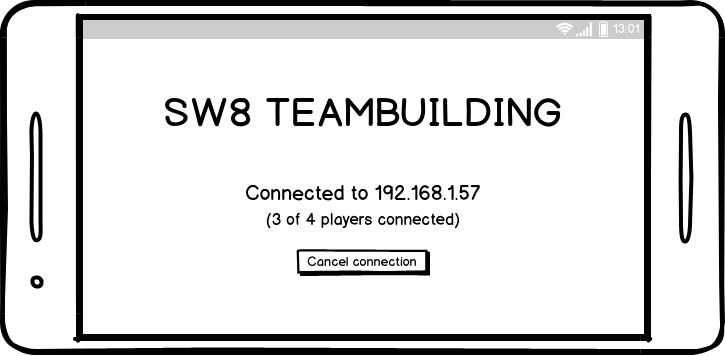
\includegraphics[width=0.6\linewidth]{prototypes/menuconnected.png}
    \caption{Prototype of screen where a user has connected to the host}
    \label{fig:prototype:menuconnected}
\end{figure}

When all users have connected, the host can start the game, and they will now see the virtual game field, as seen on \autoref{fig:prototype:ingame}.
In this prototype, the player's icon is highlighted by having a solid color, whereas the other players are just shown as outlines.
In the middle of the screen is the ball in a designated starting area to make the game fair for both teams.

\begin{figure}[H]
    \centering
    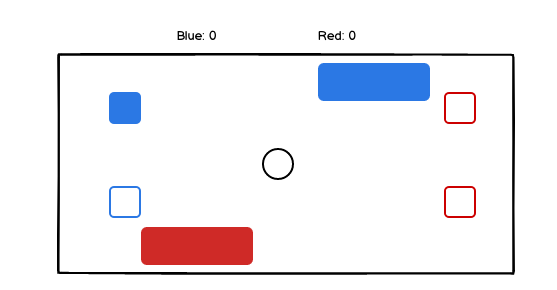
\includegraphics[width=0.6\linewidth]{prototypes/ingame.png}
    \caption{Prototype of in-game screen}
    \label{fig:prototype:ingame}
\end{figure}
